The system allows users to reserve available cars, to manage their requests and charge them for the rental.

The users can:
\begin{itemize}
\item Register to the service;
\item Login with their personal account;
\item Edit and manage personal information and delete their accounts;
\item Locate nearby available-to-rent vehicles;
\item Reserve one of said cars for a fixed amount of time;
\item Unlock the reserved vehicle based on their mobile device GPS position;
\item Alternatively, unlock the reserved car by inserting a vehicle-specific code into the application;
\item Start the engine through a to-be-defined authentication method;
\item Provide and later modify a favourite payment method for the system to manage actual due payments.
\end{itemize}
\begin{figure}[!h]
	\centering
		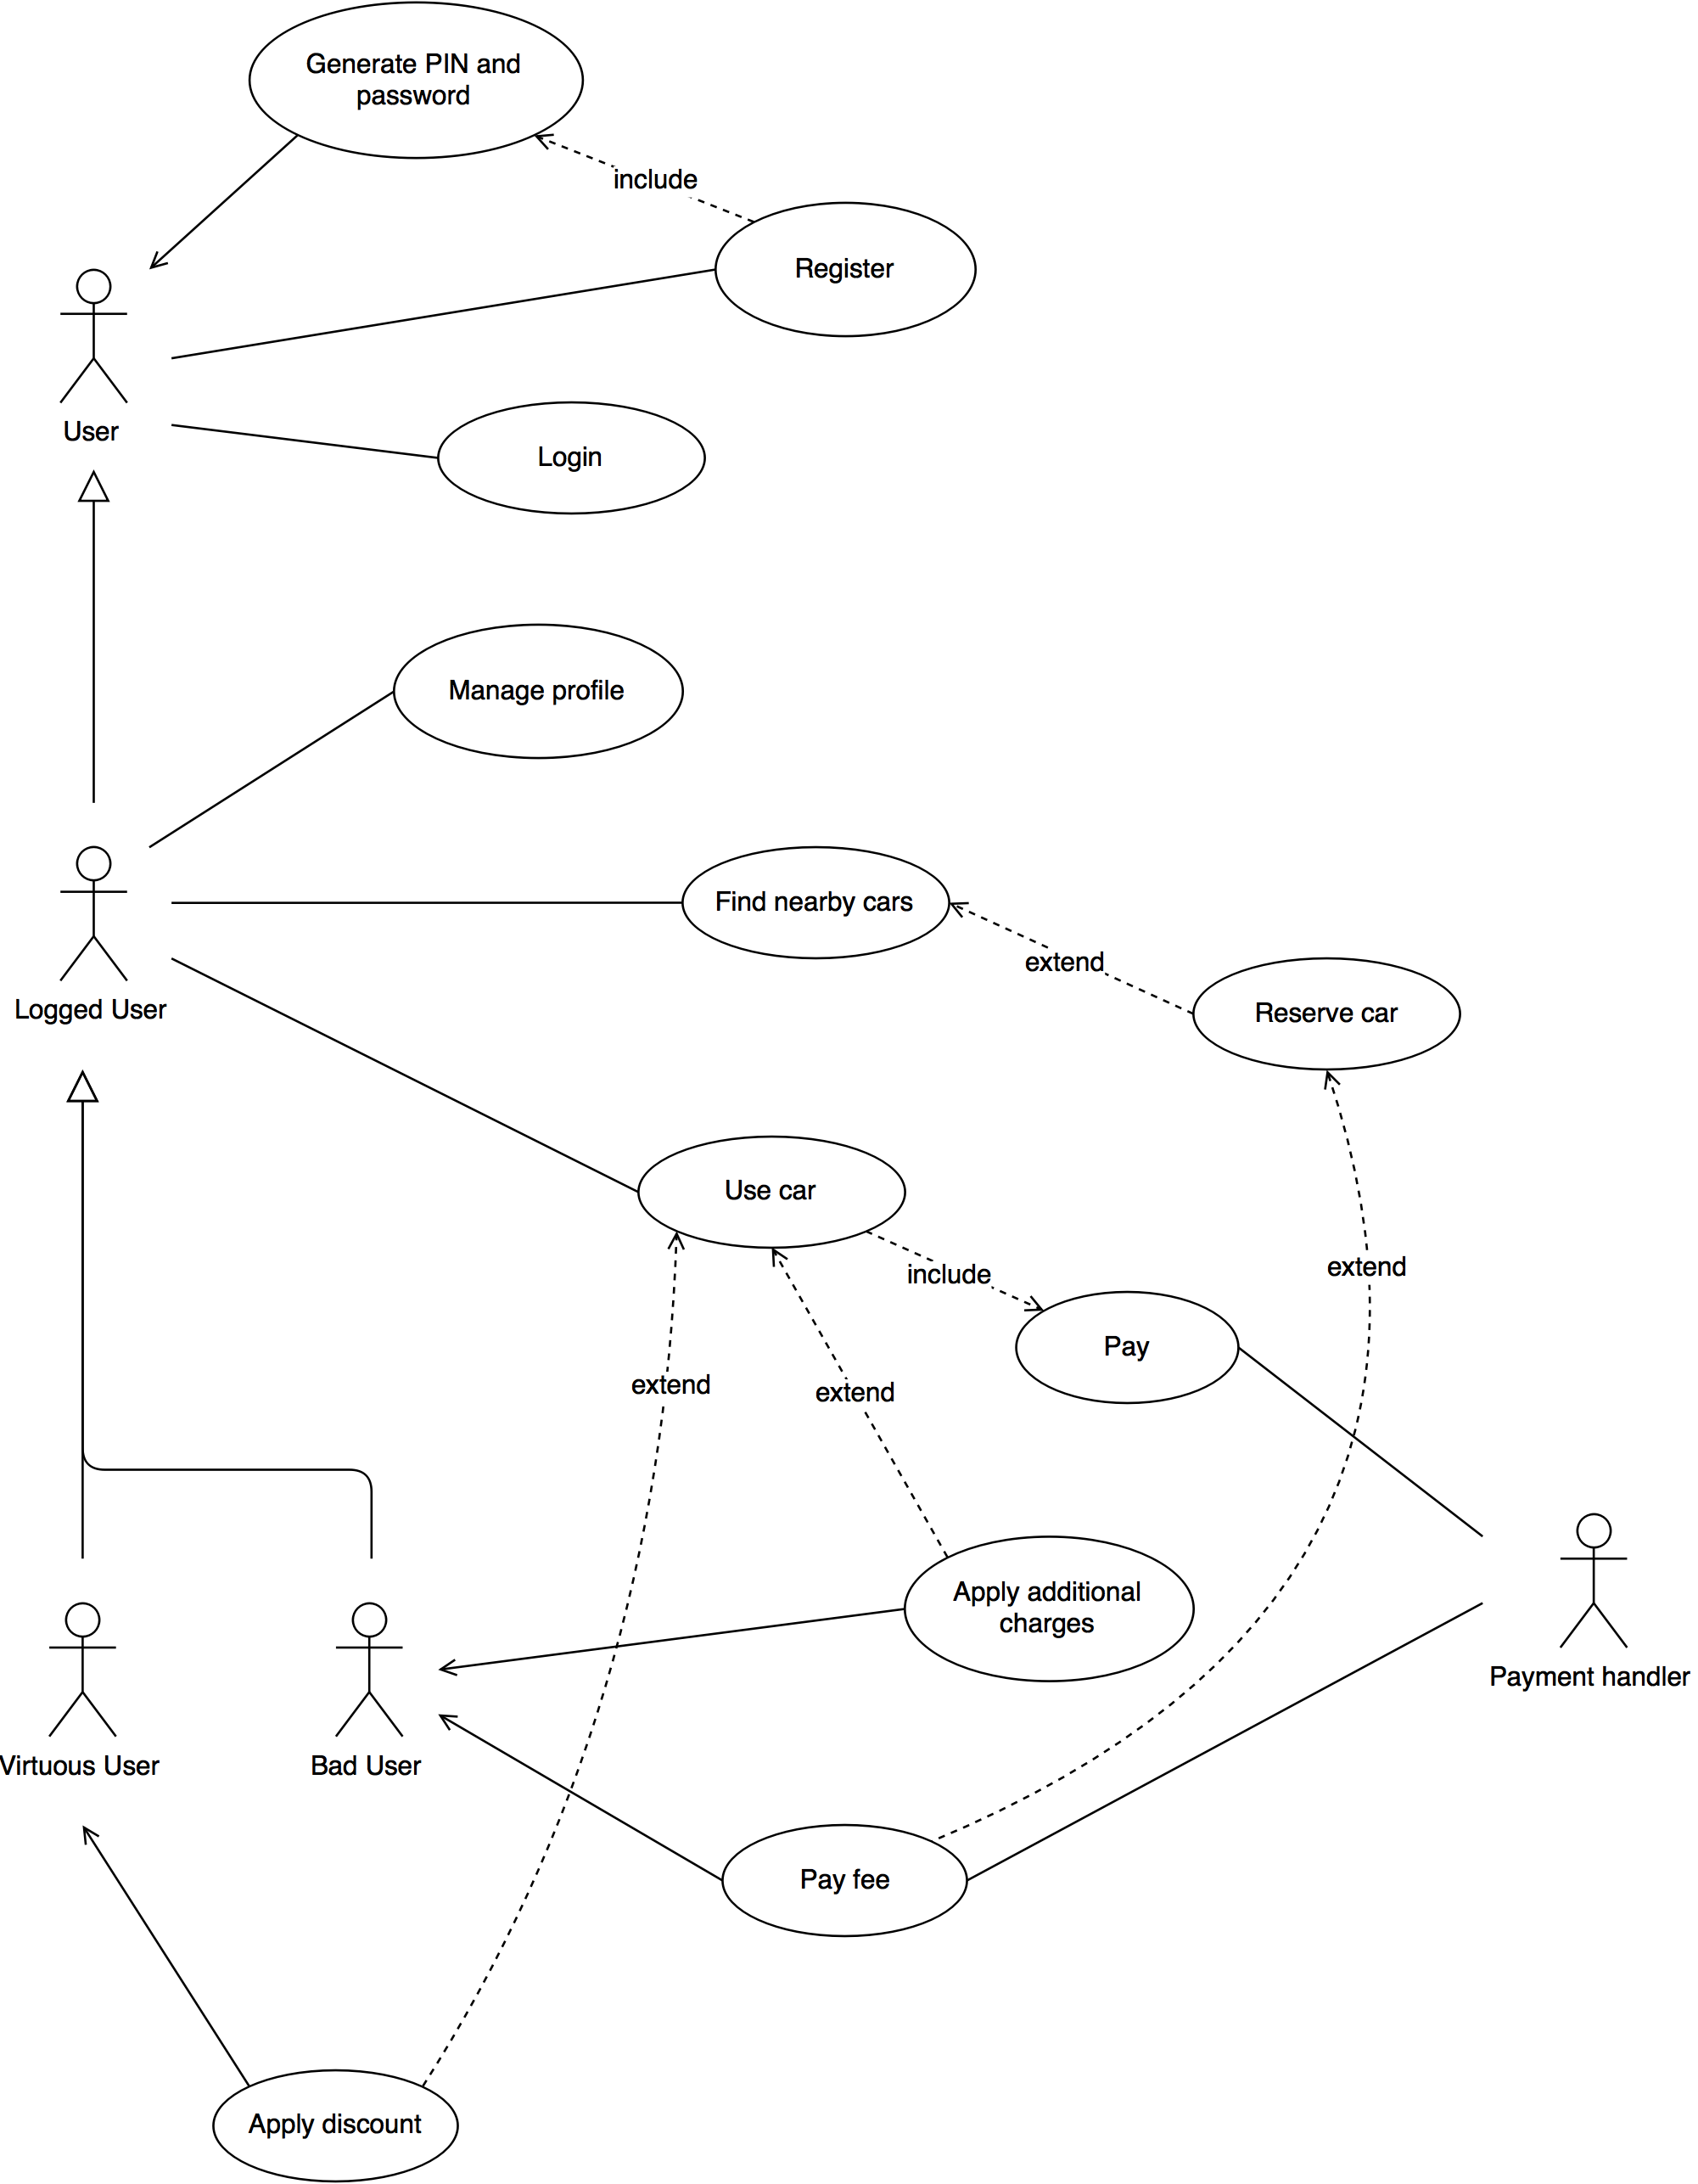
\includegraphics[width=\textwidth]{./pictures/use_case.png}
		\caption{The comprehensive use-case diagram of all the functionalities provided by the 						system.\\Note: all directed arrows from the system functions towards actor imply a notification.}
	\label{global_uc}
\end{figure}